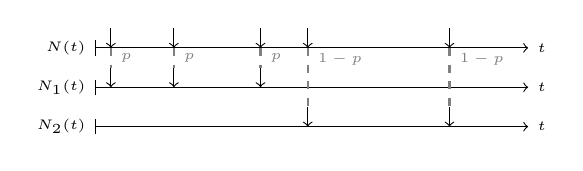
\begin{tikzpicture}
    \draw[|->]  (0,0) node[anchor=east]
        {\tiny $N(t)$}-- (5.5,0)
        node[anchor=west] {\tiny $t$};
    \draw[|->] (0,-.5) node[anchor=east]
        {\tiny $N_1(t)$} -- (5.5,-.5)
        node[anchor=west] {\tiny $t$};
    \draw[|->] (0,-1) node[anchor=east]
        {\tiny $N_2(t)$} -- (5.5,-1)
        node[anchor=west] {\tiny $t$};

    % Arrivals top
    \draw[->] (.2,0.25) -- (.2,0)
        node (first) {};
    \draw[->] (1,0.25) -- (1,0)
        node (second) {};
    \draw[->] (2.1,0.25) -- (2.1,0)
        node (third) {};
    \draw[->] (2.7,0.25) -- (2.7,0)
        node (fourth) {};
    \draw[->] (4.5,0.25) -- (4.5,0)
        node (fifth) {};


    % Arrivals mid
    \draw[thick,dashed,gray]
        (.2,0) -- (.2,-.25) node[midway,
        anchor=west] {\tiny$p$};
    \draw[->] (.2,-.25) -- (.2,-.5);
    %
    \draw[thick,dashed,gray]
        (1,0) -- (1,-.25) node[midway,
        anchor=west] {\tiny$p$};
    \draw[->] (1,-.25) -- (1,-.5);
    %
    \draw[thick,dashed,gray]
        (2.1,0) -- (2.1,-0.25) node[midway,
        anchor=west] {\tiny$p$};
    \draw[->] (2.1,-0.25) -- (2.1,-.5);
    %
    \draw[thick,dashed,gray]
        (2.7,0) -- (2.7,-0.75) node[pos=.2,
        anchor=west] {\tiny$1-p$};
    \draw[->] (2.7,-0.75) -- (2.7,-1);
    %
    \draw[thick,dashed,gray]
        (4.5,0) -- (4.5,-0.75) node[pos=.2,
        anchor=west] {\tiny$1-p$};
    \draw[->] (4.5,-0.75) -- (4.5,-1);


\end{tikzpicture}

